\input{tikz}
\begin{document}
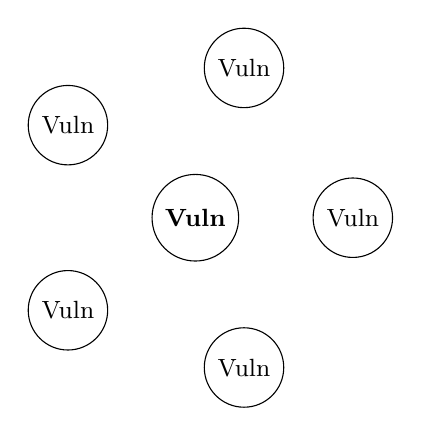
\begin{tikzpicture}

\node[draw, circle] (1) at (360/5 * 0:2cm) {\small Vuln};
\node[draw, circle] (2) at (360/5 * 1:2cm) {\small Vuln};
\node[draw, circle] (3) at (360/5 * 2:2cm) {\small Vuln};
\node[draw, circle] (4) at (360/5 * 3:2cm) {\small Vuln};
\node[draw, circle] (5) at (360/5 * 4:2cm) {\small Vuln};
\node[draw, circle] (6) at (0:0) {\textbf{\small Vuln}};

%\path [->] (1) edge node {} (6);
%\path [->] (2) edge node {} (6);
%\path [->] (3) edge node {} (6);
%\path [->] (4) edge node {} (6);
%\path [->] (5) edge node {} (6);

\end{tikzpicture}
\end{document}
